\documentclass[11pt,a4paper]{article}
\usepackage[utf8]{inputenc}
\usepackage[sfdefault]{ClearSans}
\usepackage[T1]{fontenc}
\usepackage[left=25mm,right=25mm,top=25mm,bottom=25mm]{geometry}
\usepackage[czech]{babel}
\usepackage{titling}
\usepackage{graphicx}
\usepackage{caption}
\usepackage{subcaption}
\usepackage{acronym}
\usepackage{setspace}
\usepackage{indentfirst}
\usepackage{hyperref}

\newcommand{\subtitle}[1]{%
	\posttitle{%
		\par\end{center}
		\begin{center}\large#1\end{center}
		\vskip0.5em}%
}

\graphicspath{ {./img/} }

\onehalfspacing
\setlength{\parindent}{2em}
\setlength{\parskip}{0.1em}

\title{PlantHub}
\subtitle{soutěž KYBER STOČ 2022 }
\author{Filip Sikora, Jakub Vantuch}
\date{}

\begin{document}

\begin{titlepage}
	\noindent
\includegraphics[width=\linewidth]{header.png}
	\vspace{4cm} \\
	\begin{center}
		\Huge\textbf{Zavlažovací systém PlantHub}
		\vspace{1cm} \\
		\LARGE Filip Sikora, Jakub Vantuch
		\vspace{1cm} \\
		\Large soutěž SOČ 2022
		\vfill
		\normalsize
		\begin{minipage}{0.7\linewidth}
			Třída: \textbf{4.IT}
		\end{minipage}%
		\begin{minipage}{0.25\linewidth}
			Školní rok: \textbf{2021/22}
		\end{minipage}
	\end{center}

\end{titlepage}

\section*{Prohlášení}

Prohlašuji, že jsem svou práci SOČ vypracoval/a samostatně a použil/a jsem
pouze prameny a literaturu uvedené v seznamu bibliografických záznamů.

Prohlašuji, že tištěná verze a elektronická verze soutěžní práce SOČ jsou
shodné.

Nemám závažný důvod proti zpřístupňování této práce v souladu se zákonem č.
121/2000 Sb., o právu autorském, o právech souvisejících s právem autorským a o
změně některých zákonů (autorský zákon) ve znění pozdějších předpisů.

Ve Frýdku-Místku dne 4. 3. 2022

\begin{tabular}{@{}p{2.5in}p{2.5in}@{}}
	 & \dotfill
\end{tabular}

\section*{Prohlášení}

Prohlašuji, že jsem svou práci SOČ vypracoval/a samostatně a použil/a jsem
pouze prameny a literaturu uvedené v seznamu bibliografických záznamů.

Prohlašuji, že tištěná verze a elektronická verze soutěžní práce SOČ jsou
shodné.

Nemám závažný důvod proti zpřístupňování této práce v souladu se zákonem č.
121/2000 Sb., o právu autorském, o právech souvisejících s právem autorským a o
změně některých zákonů (autorský zákon) ve znění pozdějších předpisů.

Ve Frýdku-Místku dne 4. 3. 2022

\begin{tabular}{@{}p{2.5in}p{2.5in}@{}}
	 & \dotfill
\end{tabular}

\clearpage

\section*{Anotace}

PlantHub je automatický zavlažovací systém s WUI.
Jádrem našeho systému je mikropočítač RPi s procesorovou architekturou ARM,
GPIO a možností připojení pomocí ethernetu.
Vybrali jsme si jej, protože kombinuje malou velikost a vyšší výpočetní sílu
než Arduino. Musí totiž zvládnout řídit všechny senzory, ukládat data do
databáze a zároveň hostuje i samotnou webovou aplikaci. Systém PlantHub dále
získává informace o teplotě, vlhkosti a tlaku vzduchu a promítá je ve svém
WUI. Ve stejné chvíli naměřená data ukládá do databáze v periodě 4
hodin. Jelikož voda časem z nádrže dojde systém PlantHub snímá stav hladiny
vody v nádrži a včas upozorní, že je třeba doplnit vodu.

\section*{Klíčová slova}

zavlažování; automatizace; statistika; živě; RaspberryPi; uživatelské rozhraní

\clearpage

\tableofcontents

\clearpage

\section{Úvod}

Našim cílem je návrh, sestavení a naprogramování automatického zavlažovacího
systému s WUI a ukládáním naměřených dat do databáze
pro pozdější statistiky. Tato stanice pravidelně snímá data ze senzorů měřících
teplotu a vlhkost vzduchu, vlhkost půdy a stav hladiny v nádrži, z té pak
stanice přečerpává vodu pomocí čerpadla spouštěného tranzistorem. Naměřená data
se posílají živě pomocí REST API prostřednictvím
protokolu HTTP do WUI a ve stejné
chvíli se v periodě čtyř hodin ukládají do PostgreSQL databáze běžící v docker
containeru pro pozdější
statistiky
změn teploty, vlhkosti vzduchu, vlhkosti půdy a počtů zavlažování v časovém
rozsahu zobrazitelné v dashboardu WUI. Pro načtení historických dat z databáze
používáme GraphQL API, jelikož nabízí šetrnější přístup k datům, vybráním pouze
těch záznamů z tabulky, které opravdu využíváme. V případě nedostupnosti
serveru by se ve WUI měla pořád načítat živě naměřená data z REST API. Přístup
k naměřeným datům a
WUI má pouze
uživatel lokální
sítě, do které je planthub připojen pomocí ethernet kabelu, z čehož vyplývá, že
pro správnou funkci
stanice je zapotřebí router s přístupem k internetu a DHCP serverem.

Ve WUI hostovaném na naší stanici, a sestavém pomocí javascriptového frameworku
React.js, CSS frameworku
Tailwind a programovacího jazyku Typescript, který je supersetem javascriptu,
podporujícím volitelné statické typování, má uživatel
možnost zobrazení statistik jak živě naměřených dat tak dat historických v
nastavitelných grafech dashboardu. WUI také nabízí manuální kontrolu nad
čerpadlem s časovačem začátku zavlažování a restartem hlavního programu.
Nastavitelné je jak WUI tak i samotné faktory zavlažování jako je limit
vlhkosti
půdy, doba zavlažování nebo limit hladiny vody.

Jednotlivé součásti a moduly stanice jsme vybrali podle finanční dostupnosti a
adekvátních technických
požadavků na přesnost měření.
Zapojení těchto modulů do obvodu jsme prvně provedli ve webové aplikaci
EasyEDA, která nabízí jednoduché prostředky pro návrh technických
schémat. Tento obvod jsme poté v testovací verzi postavili na nepájivém
poli a ve finální verzi navrhli a objednali vlastní PCB. Pro ochranu naší
stanice jsme v open-source programu FreeCad navrhli model krytu, který jsme
následně vytiskli na 3D tiskárně. Vymstila se nám však nepřesnost rozměrů krytu
a při vkládání stanice do krytu se nám podařilo zlomit SD kartu s operačním
systémem, daty a nasazenými programy. Po reinstalaci operačního systému jsme
opravili rozměry vytvořeného modelu krytu a
vytiskli kryt podruhé, tentokrát ve správných rozměrech.

Hlavní program jsme v prvotní verzi psali ve vysokoúrovňovém programovacím
jazyce Python, od kterého jsme nakonec upustili kvůli vysokým technickým
nárokům. Naše rozhodnutí nás nakonec dovedlo k jazyku
Go vytvořeného Googlem a určeného pro concurrency, rychlou kompilaci i průběh
programu, backend webových aplikací a mnoho
další funkcionality. Tento jazyk se nám zalíbil natolik že jsme se v něm
rozhodli
udělat jak API,
databázové funkce tak i hlavní program. Program je rozdělen na několik sekvencí
z toho hlavní jsou měřící sekvence kde se každou sekundu provádí měření dat ze
senzorů a následné odesílání na REST API webové aplikace a channely vytvořené
pro komunikaci mezi go rutinama a sekvence controlleru, která pomocí snímání
dat z databáze určuje jestli se jedná o první spuštění PlantHubu, a podle toho
určí jestli se spustí incializační sekvence nebo sekvence zavlažování.

\clearpage

\section{Hardware}

Potřebujeme vyvinout vhodné pouzdro pro naše Raspberry, abychom ochránili
citlivé elektronické součástky a ve stejné chvíli měli možnost jednoduše
vyjmout stanici z krytu. Budeme ho tisknout na 3D tiskárně pevným PTG
filamentem. K
zavlažování je potřeba postavit i nádrž na vodu, ze které bude naše čerpadlo
přečerpávat vodu k zavlažování, proto jsme se rozhodli pro nádobu s co
nejvetším objemem a postavili ji z upraveného 5L soudku.

\subsection{DHT11}

Senzor DHT11 se skládá z jednotky pro měření teploty, jednotky pro měření
vlhkosti a převodníku.

Teplotu měří senzor termistorem. Thermistor je keramický polovodič, který
zmenšuje svou rezistivitu, když se okolní teplota zvýší.

Vlhkost měří senzor na základě rezistivity substrátu umístěného mezi dvěma
elektrodami. Tento substrát zachytává vlhkost a vytváří tak vodivé prostředí

\subsection{Senzor vlhkosti půdy}

Jedná se o kapacitní senzor, ten se skládá ze dvou vodivých desek a převodníku.
Čidlo funguje na způsob kapacitoru avšak jeho kapacita je ovlivněna vlhkostí,
která ovlivňuje dielektrikum mezi dvěma deskami.

\subsection{MCP3008}

RPi má v rámci GPIO pouze digitální vstupy, protože je ale senzor vlhkosti půdy
analogový museli jsme použít ADC převodník. Přemapujeme tedy analogový signál
do
osmi různých digitálních hodnot, kterým se také říká 3bitové rozlišení, to
definuje tu nejmenší hodnotu změny, který převodník dokáže rozlišit, této
hodnotě se říká LSB (least significant bit). ADC poté pomocí SAR
definuje adresu v binárním podání srozumitelným pro digitální vstup.

\begin{figure}[h]
	\centering
	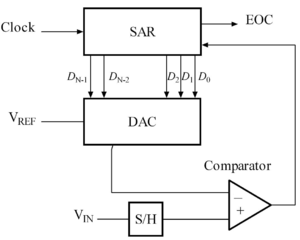
\includegraphics[width=8cm]{sar_adc.png}
	\caption{SAR}
\end{figure}
\subsection{HC-SR04}

HC-SR04 vydává zvukové vibrace na vysoké frekvenci, neslyšitelné pro lidské
ucho. Poté čeká, až se zvuk odrazí zpět, a vypočítá vzdálenost na základě času
měřeného od vysílání zvukové vlny k zpětnému přijmutí

Všechny naměřené údaje jsou v převodníku senzoru přepočítány na jednotky dané
veličiny a odeslány analogovým signálem do řídící jednotky.

\subsection{Čerpadlo}

Naše zvolené čerpadlo se skládá z DC motoru, na němž je upevněna centrifuga pro
čerpání vody a vlastního pouzdra, z kterého vede otvor pro napojení odtokové
hadičky. Čerpadlo je připojeno na zdroj napětí 5V a zem.

\subsection{2N2222}

Protože samotný signální pin neposkytuje dostatečné napětí pro chod čerpadla
ovládáme jej NPN tranzistorem. Díky našemu vyměnitelnému připojení modulů je
možné čerpadlo vyměnit a přívodný kabel používat jako spouštěč čerpadla
jakéhokoliv výkonu a nároků na zdroj.

\clearpage

\section{Obvod}

Testovací verzi našeho obvodu jsme postavili na nepájivém kontaktním poli,
které jsme používali pouze v testovací verzi. Jakmile jsme měli vše plně
odzkoušeno a plně otestováno přešli jsme na profesionálnější řešení.
Což tedy v druhé fázi znamenalo sestrojit a nechat vytisknout náš vlastní obvod
přepracovaného schématu PCB a vytisknutého společnosti JLCPCB na naše vlastní
náklady.

\begin{figure}[h]
	\centering
	\begin{subfigure}[b]{0.4\linewidth}
		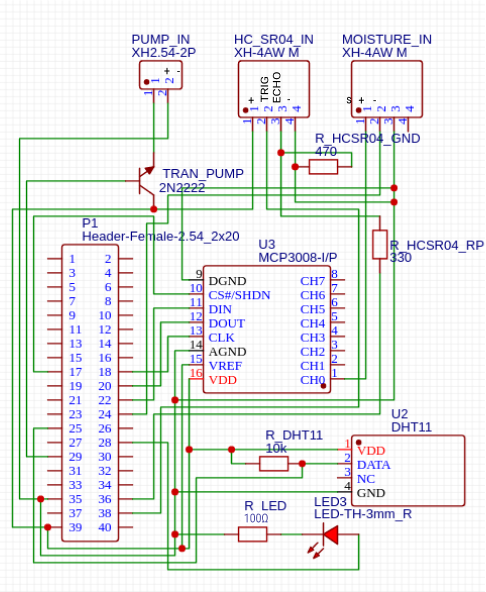
\includegraphics[width=\linewidth]{pcb.png}
		\caption{Diagram PCB}
	\end{subfigure}
	\begin{subfigure}[b]{0.4\linewidth}
		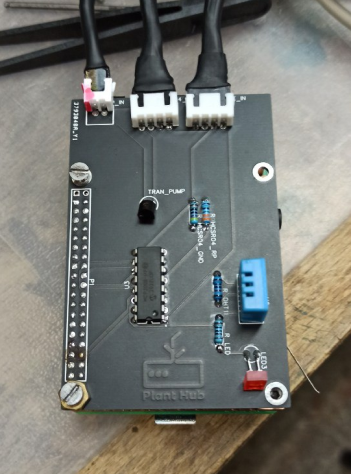
\includegraphics[width=\linewidth]{planthub.png}
		\caption{PlantHub PCB se senzory}
	\end{subfigure}
	\caption{}
\end{figure}

\clearpage

\section{Hlavní program}

\subsection{Postup práce}

Náš hlavní program pro zavlažování a komunikaci s databází a WUI
jsme začali psát ve vysokoúrovňovém programovacím jazyce Python. Od toho jsme
ale nakonec upustili kvůli pomalejšímu průběhu programu, proto jsme přešli na
programovací jazyk GO.

\begin{figure}[h]
	\centering
	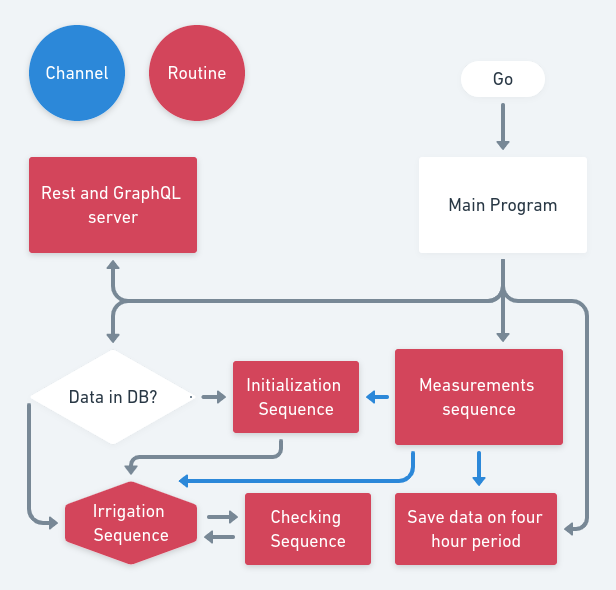
\includegraphics[width=8cm]{go.png}
	\caption{Vývojový diagram programu}
\end{figure}

\subsection{Fáze programu}

Fáze programu se spouštějí buďto v samostatné go rutině a komunikují spolu
pomocí channelů nebo na základě podmínek kde se po splnění požadavků ukončí.

\subsubsection{Měření}

Senzor vlhkosti půdy a DHT11 průběžně posílají naměřená data do Rpi, kde se
ukládají do databáze. Jestliže naměřené hodnoty překročí limitní hodnoty, Rpi
pošle signál pro otevření tranzistoru což spustí čerpadlo.

\subsubsection{Periodické ukládání dat}

V samostatné rutině běží funkce pro ukládání naměřených dat v periodě 4 hodin.
Naměřená data jsou následně statisticky zobrazena v UI.

\subsubsection{Controller}

Po spuštění měřící sekvence a sekvence periodického ukládání dat se spustí
buďto incializační sekvence a nebo zavlažovací sekvence podle toho jestli jsou
v databázi data nastavení, nastavovaná ve WUI. Pokud data nejsou tak program
čeká na uložení dat z WUI a LED dioda bliká dvakrát po sobě dokud data nejsou
dostupná, pokud ano spustí se zavlažovací sekvence, načtou se limitní data z
databáze a v periodě 1 sekundy se budou číst data o vlhkosti půdy.

\subsubsection{Inicializace}

Půda musí být ze začátku suchá. Senzor vlhkosti půdy zasuneme co nejhlouběji do
půdy. Rpi bude chvíli sbírat data a pak je zprůměruje do hodnoty, která bude
sloužit jako limit pro spuštění čerpadla.

V UI jde navíc ještě manuálně nastavit hranice vlhkosti půdy pro spuštění
čerpadla.

Nastavit se dá také množství vody, které bude přečerpáno při jednom spuštění a
jaká je hranice pro přijatelnou výšku hladiny vody v nádrži. Pokud nejsou tyto
hodnoty uvedeny čerpadlo bude vodu přečerpávat, dokud se nezmění hodnota
kapacitního čidla pro měření vlhkosti půdy a HC-SR04 použije výchozí nastavení.

\subsubsection{Zavlažování}

Čerpadlo začne čerpat vodu a zavlažovat rostlinu. Voda se čerpá tak dlouho,
dokud senzor vlhkosti půdy nezmění svou hodnotu nebo dokud není vyčerpán limit
přečerpané vody na jedno spuštění.

\subsubsection{Kontrola}

Po ukončení přečerpávání se spustí HC-SR04 a změří výšku hladiny vody. Naměřená
data poté odešle do Rpi kde se uloží do databáze. Pokud bude naměřená hodnota
nižší, než je limitní hodnota, začne blikat LED dioda a Rpi odešle upozornění o
doplnění nádrže do UI. Jakmile bude hladina doplněna, signalizace se vypne.

\subsection{Ukládání dat}

Náš systém ukládá zvlášť periodicky naměřená data a data naměřená před
zavlažováním, dále ukládá nastavení jak pro limity k zavlažování, tak pro
WUI.

\clearpage

\section{WUI}

Webovovou aplikaci jsme napsali pomocí javascriptového frameworku
React.js, CSS frameworku
Tailwind a programovacího jazyku Typescript, který je supersetem javascriptu,
podporujícím volitelné statické typování. Ve webovém rozhraní je možné zobrazit
si statisky jak živě
naměřených dat, tak dat uložených v databázi. Z OpenWeather API získáváme data
o předpovědi počasí a do dahsboardu renderujeme předpovědi na dalších 15H.

\begin{figure}[h]
	\centering
	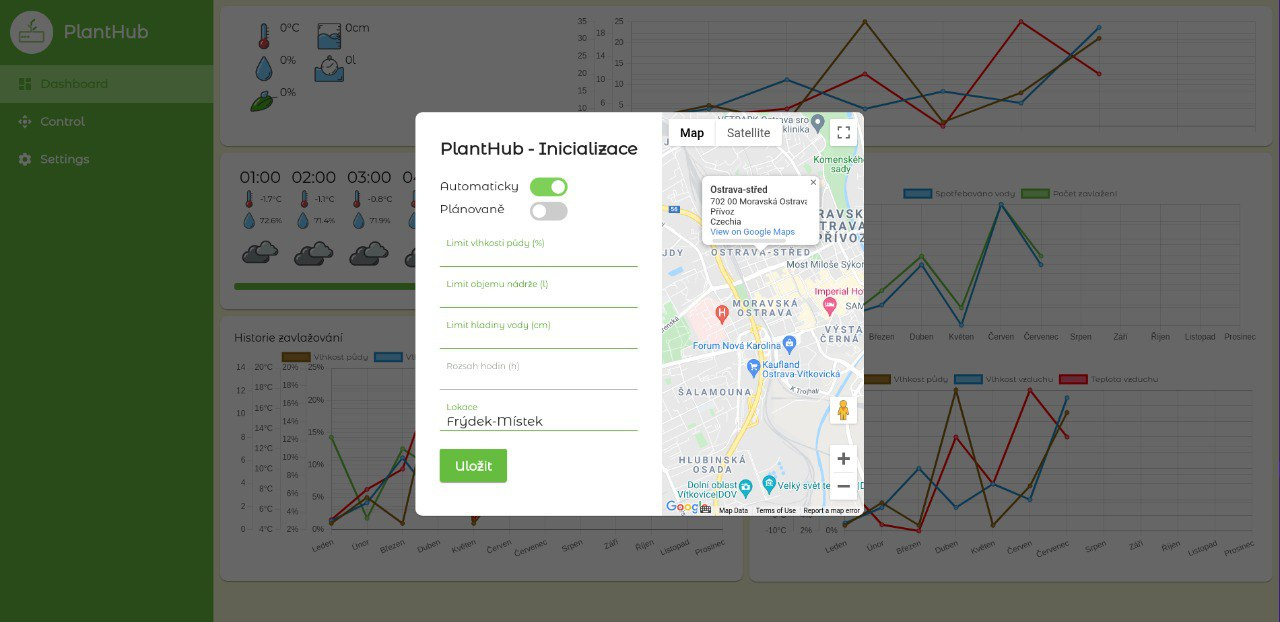
\includegraphics[width=0.9\linewidth]{ui-inicializace.jpg}
	\caption{Okno prvotního nastavení. Nastaví se zde limity a celkové
		nastavení aplikace.}
\end{figure}

\begin{figure}[h]
	\centering
	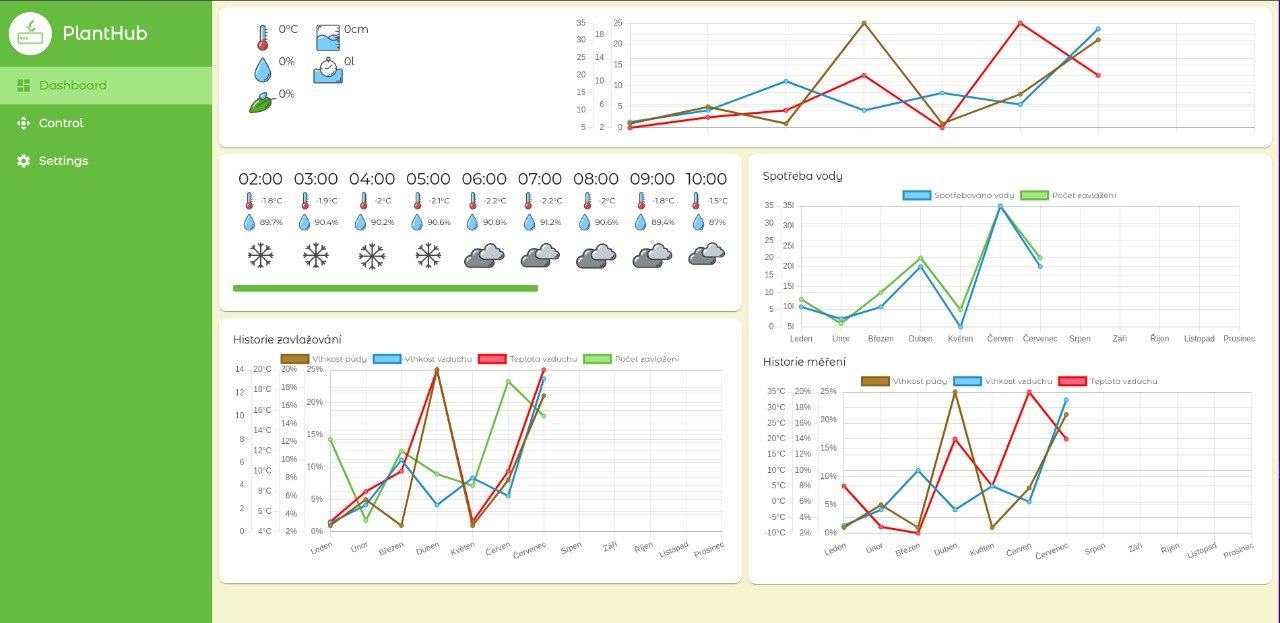
\includegraphics[width=0.9\linewidth]{web-ui.png}
	\caption{Dashborad WUI}
\end{figure}

\begin{figure}[h]
	\centering
	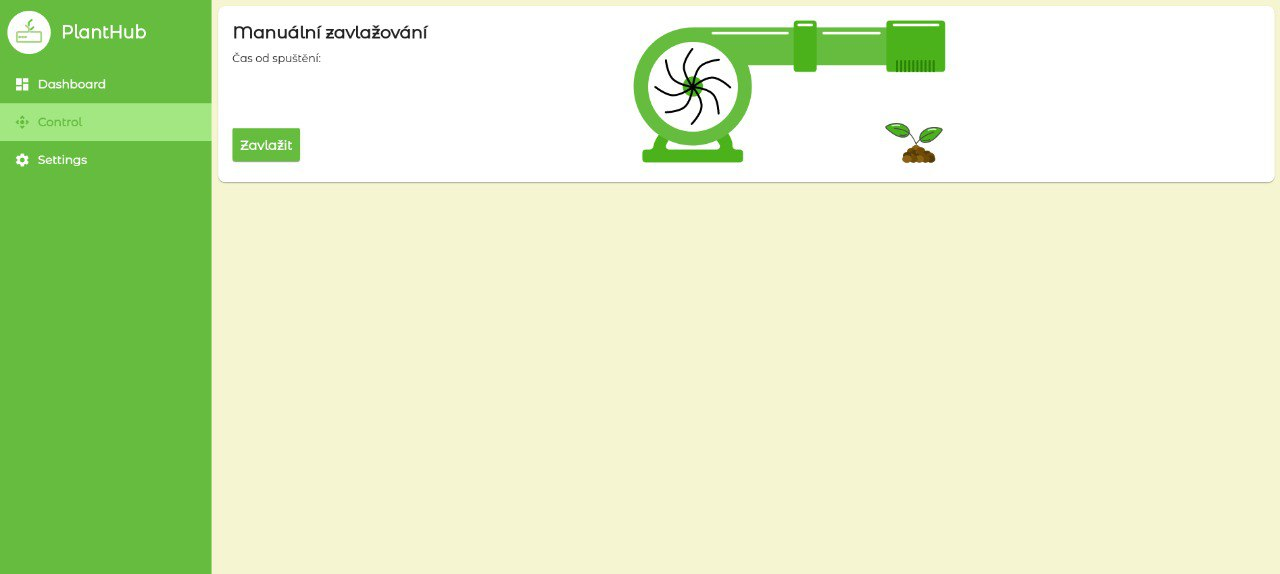
\includegraphics[width=0.9\linewidth]{web-ui-pump.png}
	\caption{Interaktivní ovládání celého systému lze provést v již
		zmiňované webové aplikaci. Dovoluje uživateli kdykoliv spustit
		čerpadlo na
		zalévání rostliny.}
\end{figure}

\begin{figure}[h]
	\centering
	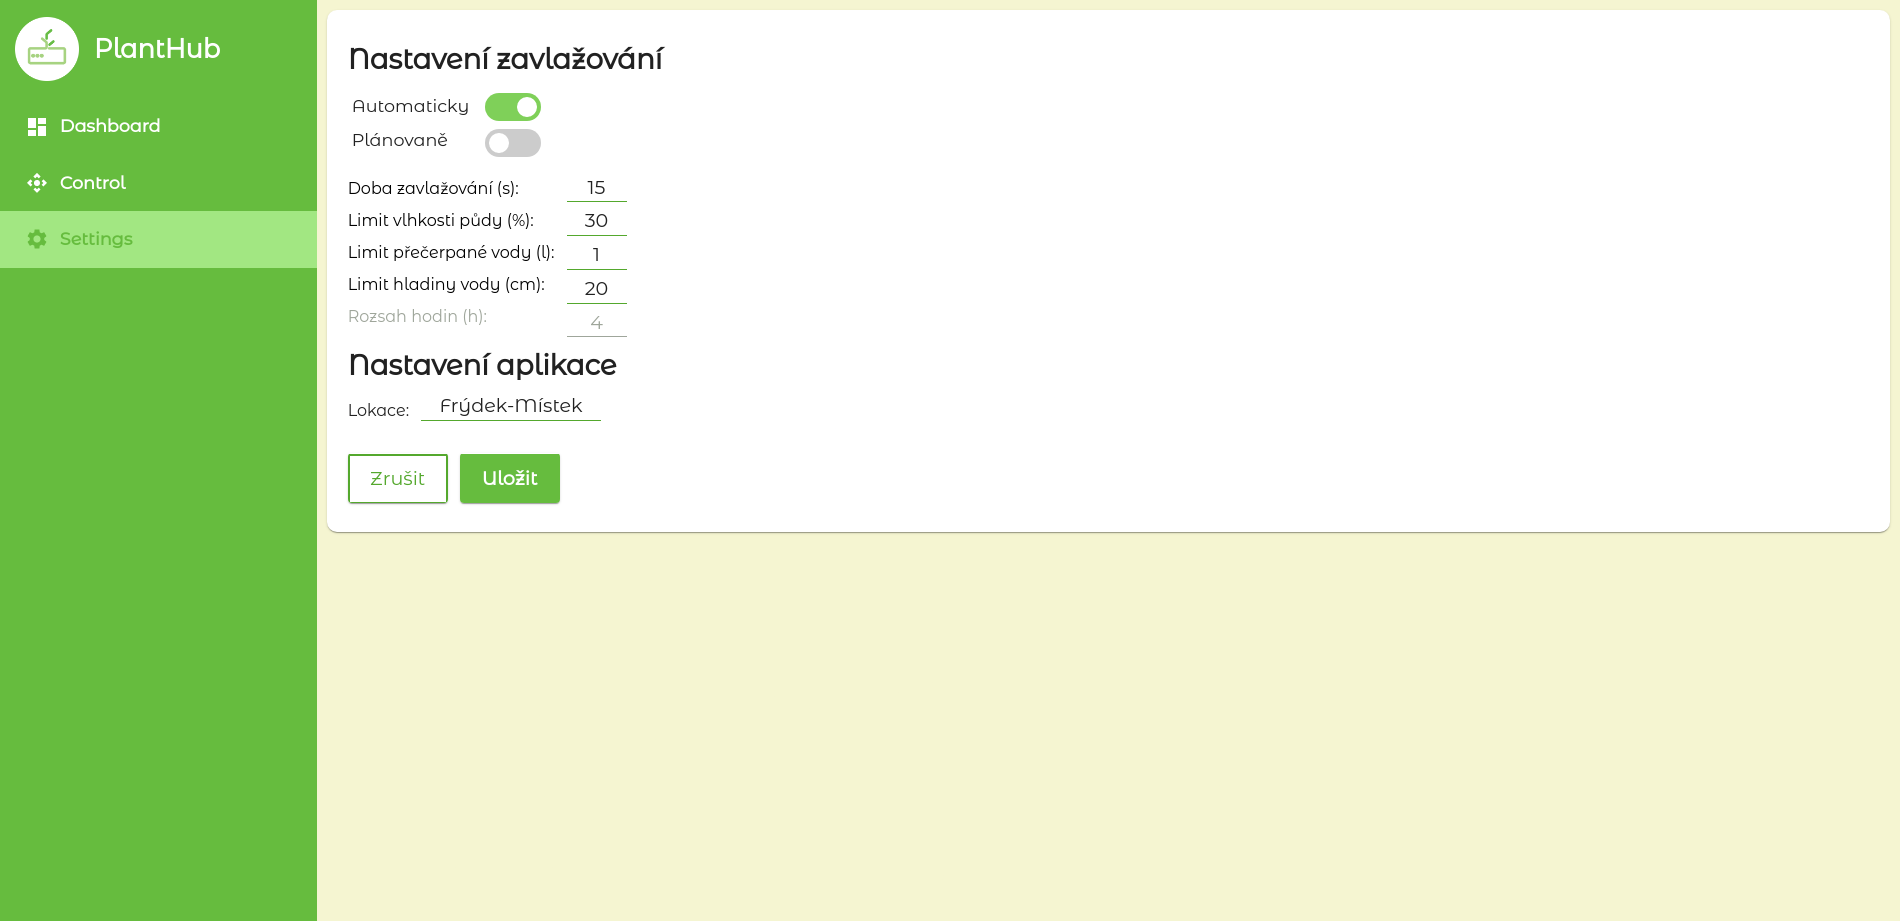
\includegraphics[width=0.9\linewidth]{web-ui-settings.png}
	\caption{V nastavení se dá změnit nastavení aplikace i limitů pro
		zavlažování. Nastavení se poté uloží do databáze.}
\end{figure}

\clearpage

\section{Databáze}

Pro databázi jsme se rozhodli použít databázový systém PostgreSQL. Jak vyplývá
z názvu, jedná se o SQL databázi, ty jsou vhodné pro ukládání velkého objemu
dat, jako právě data z našich senzorů. Webová aplikace používá pro přístup k
datům z databáze GraphQL API.

GraphQL je query, který je konkurent řešení REST API. Nabízí efektivnější
tvorbu API a také umožňuje efektivnější přístup k datům z databáze. Umožňuje
vybrat pouze data, která momentálně aplikace používá a dovoluje vynechat data,
která zrovna potřebné nejsou.

\clearpage

\section{Webový server}

Web server jsme napsali v moderním jazyku Go, který nyní roste v popularitě
hlavně mezi cloudovými vývojáři a v oblasti vývoje microservices. Dokáže se
exekuční rychlostí přiblížit k nízkoúrovňovým jazykům jako je C nebo Rust, ale
zároveň zůstává velmi lidsky čitelný a jednoduchý na použití. Na rozdíl od
jazyků jako C a Rust má například garbage collector.

\clearpage

\section{Na čem ještě pracujeme}

\begin{itemize}
	\item RPi case z 3D tisku
	\item Celková funkcionalita hlavního programu a jeho sekvencí
	\item Realizace nádrže pro vodu
\end{itemize}

\begin{figure}[h]
	\centering
	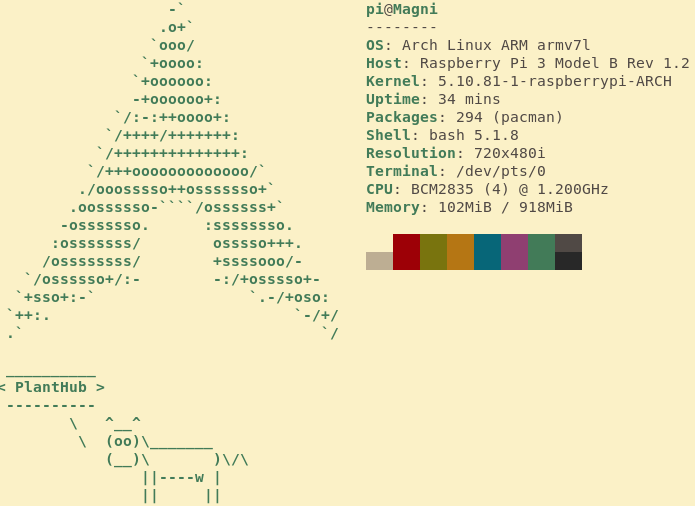
\includegraphics[width=0.7\linewidth]{specs.png}
	\caption{Specifikace RaspberryPi}
\end{figure}

\clearpage

\section{Závěr}

Filip Sikora je kokor.

\clearpage

\section{Seznam zkratek a pojmů}

\begin{acronym}
	\acro{WUI}{Webové uživatelské rozhraní}
	\acro{API}{Application programming interface}
	\acro{REST}{Representaion programming interface}
	\acro{GraphQL}{Graph query languge}
	\acro{PCB}{Printed circuit board}
	\acro{RPi}{Raspberry Pi}
	\acro{ARM}{Advanced RISC Machines}
	\acro{GPIO}{General-purpose input/output}
	\acro{DHT11}{Digital humidity temperature (sensor) v.11}
	\acro{HC-SR04}{Ultrasonický senzor vzdálenosti}
	\acro{MCP3008}{Analog-digital converter}
	\acro{Cerpadlo}{Ponorné mini čerpadlo eses}
	\acro{2N2222}{NPN tranzitor}
	\acro{SPI}{Serial peripheral interface}
	\acro{SAR}{Successive-approximation}
\end{acronym}

\clearpage

\section{Použité nástroje}

\begin{acronym}
	\acro{Code-OSS}{Open-source verze známého textového editoru Visual
		Studio Code.}
	\acro{GoLand}{Inteligentní IDE vyvinuté společností
		JetBrains speciálně pro jazyk Go.}
	\acro{Git}{Software pro tracking změn souborů repozitáře projektu
		uloženého na GitHubu.}
	\acro{Figma}{Webová aplikace pro tvoření vektorové grafiky a návrhů
		uživatelských rozhraní.}
	\acro{FreeCad}{Open-source program pro modelování 3D objektů.}
	\acro{EasyEDA}{Webová aplikace nabízející jednoduché
		prostředky pro návrh technických
		schémat}
\end{acronym}

\clearpage

\section{Použité zdroje}
\href{http://www.latex-tutorial.com}{LaTeX-Tutorial}.
\newline
\href{http://www.freecodecamp.org}{Free Code Camp}.
\newline
\href{http://www.go.dev}{Go lang}.
\newline
\href{http://www.reactjs.org}{React.js}.
\newline
\href{http://www.tailwindcss.com}{Tailwind CSS}.
\newline
\href{http://www.typescriptlang.org}{Typescript}.
\newline
\href{https://www.kali.org/tools/code-oss}{Code-OSS}.
\newline
\href{https://www.jetbrains.com/go/}{Goland}.
\newline
\href{https://git-scm.com/}{Git}.
\newline
\href{https://www.figma.com/}{Figma}.
\newline
\href{https://www.freecadweb.org/}{FreeCad}.
\newline
\href{https://componentsearchengine.com/library/easyeda}{EasyEDA}.

\clearpage

\section{Seznam obrázků}

\begin{acronym}
	\acro{Obrázek 1. }{SAR}
	\acro{Obrázek 2. (a)}{Diagram PCB}
	\acro{Obrázek 2. (b)}{PlantHub PCB se senzory}
	\acro{Obrázek 3.}{Vývojový diagram projektu}
	\acro{Obrázek 4.}{Okno prvotního nastavení WUI}
	\acro{Obrázek 5.}{Dashboard WUI}
	\acro{Obrázek 6.}{Manuální ovládání z WUI}
	\acro{Obrázek 7.}{Nastavení PlantHubu a WUI}
	\acro{Obrázek 8.}{Specifikace RaspberryPi}
\end{acronym}

\clearpage

\section{Seznam příloh}

\end{document}